\subsection{Analizador de figura de ruido N8975A (NFA Series Noise Figure Analyzer)}
\subsubsection{Descripción general}

Representa el equipo fundamental en el sistema de la figura 2, es esencialmente un dispositivo que mide de potencia de ruido en RF y UW generada por elementos pasivos o activos. A partir de la medida de potencia, este equipo puede	calcular el valor de la figura de ruido de elemento, así como también su temperatura efectiva, ganancia y presentar el resultado en pantalla. 

El NFA mide la potencia total de ruido que genera un dispositivo bajo prueba (DUT por sus siglas en inglés) cuando en su entrada se inyecta una señal de ruido de referencia. Esta señal es producida por una fuente de ruido estándar, sus características de ruido deben ser conocidas con elevada exactitud. En el sistema CENDIT, se emplean las fuentes de ruido de la serie Agilent N4000A. La fuentes de ruido N4000A son conocidas como fuentes de ruido inteligentes, ya que	estas almacenan en una memoria no volátil interna, una tabla que caracteriza su potencia de ruido en función de la frecuencia, conocida como tabla de ENR. Además, cuentan con un sensor de temperatura integrado.

A través de un cable que conecta el NFA con el puerto de control de la NS, el NFA puede cargar las tablas de ENR de las fuentes de ruido. De la misma forma, puede leer la temperatura de la fuente de ruido.

\begin{figure}[h!]
	\centering
	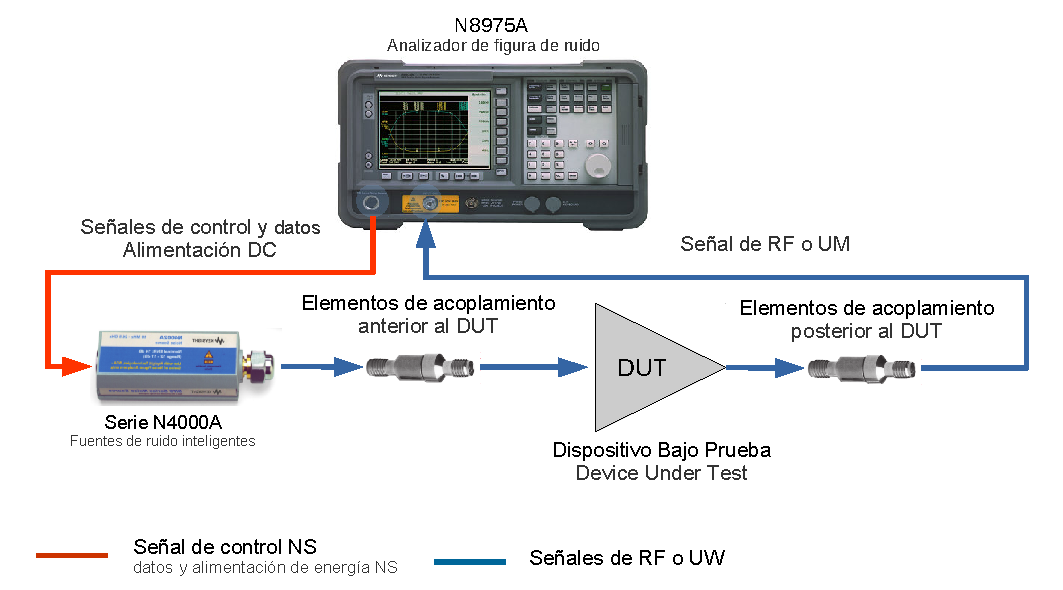
\includegraphics[width=15cm]{./Imagenes/EsquemaConexionNFADUT.pdf}
	\caption{Esquema de conexiones de la instrumentación básica para medición de NF.}
\label{Fig:BancoPruebasFuenteRuido}
\end{figure}

El N8975 emplea la técnica del factor Y para la medición de ruido sobre un DUT. Esta técnica consiste básicamente en	inyectar en la entrada del DUT dos niveles distintos de potencia de ruido, el primero   sensiblemente mayor que el segundo, para luego medir la potencia de ruido que a la salida del DUT existen para cada uno de estos niveles.	Calculado un cociente entre el valor mayor y el valor menor de la medición, esto es el factor Y, y con la tabla de	ENR de la fuente de ruido se puede conseguir la figura del ruido del DUT.

Aparte de la figura de ruido, puede realizar las siguientes mediciones:

\begin{itemize}
	\item Potencia de ruido, fría PCOLD y caliente PHOT
	\item Temperatura equivalente de ruido.
	\item Factor Y.
	\item Ganancia.
\end{itemize}

El NFA cuenta con las siguientes interfaces

\begin{itemize}
	\item Una interfaz de usuario, en su panel frontal. 
	\item Una interfaz de señal (RF y {}W)
	\item Una interfaz de datos.
\end{itemize}

La interfaz de usuario se divide a su vez en dos interfaces: interfaz local e interfaz remota. La interfaz local permite al usuario operar el NFA en sitio, la constituye el panel frontal del equipo el cual cuenta con una pantalla LCD y un conjunto de botones agrupados en bloques de acuerdo a su funcionalidad y un teclado numérico.

El monitor LCD es a color, de 17 cm, en el se presentan los datos ya se en formato de gráfico, tabla o modo de medidor.Puede presentar dos gráficas simultaneas, en estas se pueden agregar cuatro marcadores o cursores y dos lineas limites. Puerto paralelo, 25 pines D-sub, dedicado a impresora. Salida VGA conector 15 pines, mini D-sub, hembra.

El NFA dispone de la capacidad para ser operado de forma remota. En su panel trasero cuenta con un conector IEEE-488 para bus GPIB y un conector RS-232 D-sub de 9 pines. El conector IEEE-4888 permite conectar el equipo a un bus GPIB y establecer una red de instrumentos de medición. Es posible además conectar el puerto GPIN del NFA a un computador, por medio de una tarjeta como las del tipo PCI-GPIB y cable de bus GPIB empleando o un adaptador USB-GPIB. A través de bus GPIB y empleando aplicaciones de software se le envían comandos al equipo que permiten controlarlo y obtener datos de mediciones.

Interfaz GPIB conector IEEE-488, bus serial RS-232, 9 pines D-sub, macho.	
La interfaz de señal señal que dispone el equipo en su panel frontal consiste en 

\begin{itemize}
	\item Un conector de entrada para señal RF-$\mu${\textmu}F. 
	\item Un conector de salida para el control, alimentación y datos de una fuente inteligente de ruido (SNS) de la serie N4000 de Agilent 
	\item Un puerto para alimentación y conmutación de una fuente de ruido tradicional serie 346 de Agilent. 
\end{itemize}
EL conector de entrada para señal de RF / UW es de tipo APC 3.5 (m), con \ impedancia nominal de 50 Ω, ESD sensible. La potencia máxima admisible en la señal de entrada es de 10 dBm. La máxima protección de entrada ± 20V, +15dBm pico (o promedio) en RF. El rango de frecuencia admisible por ele equipo es de 10 a 26.5 GHz.

En el conector SNS se conecta una fuente de ruido SNS, a través de un cable multihilo cilíndrico. Por medio de este puerto el equipo enviá y recibe los datos almacenados de ENR y temperatura medida por la NS además de la señal de alimentación que permite conmutar la potencia de ruido generada por la SNS, las señales de alimentación y datos. 

\subsubsection{Interfaz eléctrica}

Rango de frecuencia: 10 a 26,5 GHz

Ancho de banda de medición: 4 MHz, 2 MHz, 1 MHz, 400 kHz, 200 kHz, 100 kHz.

El desempeño depende del ENR de la fuente empleada	

\begin{table}
	\centering
	\begin{tabular}{ccccc}
		\toprule
		\multicolumn{2}{c}{\bfseries Rango de ENR para la fuente   de ruido} &
		{\bfseries 4 - 7 \si{\decibel}} & 
		{\bfseries 12 - 17 \si{\decibel}} & 
		{\bfseries 20 - 22 \si{\decibel}} \\
		\midrule
		\multirow{2}{*}{\bfseries 10 \si{\mega\hertz} a 3 \si{\giga\hertz}} & {\bfseries Rango de medición} 
		& 0 a 20 \si{\decibel} 	& 0 a 30 \si{\decibel} & 0 a 35 \si{\decibel} \\
		\cmidrule{2-5}
		& {\bfseries Incertidumbre} 
		& $\pm$ < 0.05 \si{\decibel} 
		& $\pm$ < 0.05 \si{\decibel} 
		& $\pm$ < 0.1 \si{\decibel} \\
		\midrule
		\multirow{2}{*}{\bfseries Mayor a 3.0 \si{\giga\hertz}} 
		& {\bfseries Rango de medición} 
		& 0 a 20 \si{\decibel} 	
		& 0 a 30 \si{\decibel} 
		& 0 a 35 \si{\decibel} \\
					\cmidrule{2-5}
		& {\bfseries Incertidumbre} 
		& $\pm$ < 0.15 \si{\decibel} 
		& $\pm$ < 0.15 \si{\decibel} 
		& $\pm$ < 0.2 \si{\decibel} \\	
		\bottomrule	
		
	\end{tabular}
	\caption{Figura de ruido N8975A}
	\label{Tab: FiguraRuidoN8975A}
\end{table}

\begin{table}
	\centering
	\begin{tabular}{ccccc}
		\toprule
		\multicolumn{2}{c}{\bfseries Rango de ENR para la fuente   de ruido} &
		{\bfseries 4 - \SI{7}{\decibel}} & 
		{\bfseries 12 - \SI{17}{\decibel}} & 
		{\bfseries 20 - \SI{22}{\decibel}} \\	
		\midrule
		\multirow{2}{*}{\bfseries \SI{10}{\mega\hertz} a \SI{3} {\giga\hertz}} 
			& {\bfseries Rango de medición} 
		& \multicolumn{3}{c}{-20 a \SI{+40}{\decibel}} \\
		\cmidrule{2-5}			
		& {\bfseries Incertidumbre} 
		& \multicolumn{3}{c}{$\pm$ < 0.17} \\		
		\midrule
		\multirow{2}{*}{\bfseries Mayor a \SI{3.0}{\giga\hertz}} 
			& {\bfseries Rango de medición} 
		& \multicolumn{3}{c}{-20 a \SI{+40}{\decibel}} \\
		\cmidrule{2-5}			
		& {\bfseries Incertidumbre} 
		& \multicolumn{3}{c}{$\pm$ < 0.17} \\				
		\bottomrule
	\end{tabular}
	\caption{Ganancia N8975A}
\end{table}

\begin{table}
	\begin{tabular}{ccc}
		\toprule
		\textbf{Frecuencia (\si{\giga\hertz})}
		& \textbf{Figura de ruido (\si{\decibel})} 
		& \textbf{Figura de ruido @ 23 $\pm$ \SI{3}{\degreeCelsius} (\si{\decibel})} \\
		\midrule
		\textbf{0.010 a < 0.5} 
		& $< 4.9 + (0.0025)f(\si{\mega\hertz})$
		& $< 4.4 + (0.0025)f(\si{\mega\hertz})$ \\
		\textbf{0.5 a 2.3} 
		& $< 4.9 + (0.00135)f(\si{\mega\hertz})$
		& $< 5.9 + (0.00135)f(\si{\mega\hertz})$ \\
		\textbf{2.3 a < 3.0} 
		& $< 4.9 + (0.0015)f(\si{\mega\hertz})$
		& $< 2.9 + (0.0015)f(\si{\mega\hertz})$ \\		
		\textbf{3.0 a 13.2} 
		& $< 12.0$
		& $< 10.5$ \\		
		\textbf{13.2 a 26.5} 
		& $< 16.0$
		& $< 12.5$ \\		
		\bottomrule				
	\end{tabular}
\end{table}


Ruido generado por el instrumento \cite{AGI01}



	El NFA puede realizar mediciones en un rango de frecuencia o en una frecuencia particular. Si se trata de un rango o	lista de frecuencias, el dispositivo calcula la edición requerida de forma automáticas para cada valor de frecuencia de interés. El usuario también puede configurar el NFA para ejecutar la medición en forma manual en cada punto de frecuencia. 
	
	El NFA puede presentar los resultados en forma de gráficas o tablas, con el valor de la medición en función de la frecuencia. Puede almacenar y recuperar los datos de mediciones en su memoria interna.
	
	Dispone este equipo en su panel trasero de puerto 
	
	La capacidades del N8975A pueden entenderse mejor examinando el panel frontal del equipo. En la figura se muestra el panel frontal, el cual esta dividido cuatro grandes grupos de acuerdo a la funcionalidad: MEASURE, CONTROL, SYSTEM, DISPLAY.
	
	MEASURE establece los parámetros que controlan la medición coo el rango de frecuencia, el ancho de banda y la cantidad	de puntos de medición.
	
	CONTROL configura parámetros más avanzados de la medición como compensar las perdidas de elementos auxiliares y agregar lineas limite.
	
	SYSTEM configuración del sistema como la dirección GPIB del NFA, mostrar información de estado y controlar un oscilador externo.
	
	DISPLAY periten ajustar las características de la presentación de los datos que mide el instrumento, permite escoger que	parámetros mostrar y permite ajustar la escala de los gráficos.
			

	\clearpage
	\subsubsection{Interfaz de usuario. Resumen del panel frontal}
	Para realizar mediciones en modo local el usuario debe interactuar con el panel frontal, este le brinda acceso a todas las capacidades del NFA, describe por si misma todas las capacidades. Las teclas que típicamente tienen un mayor uso cuando se desarrolla una medición tienen \ mayor ancho y se ubican cerca de la parte derecha del display, están organizadas de tal forma que describen parte de la secuencia a seguir en la medición: (Frequency / Points, Averaging	/ Bandwidth, Calibrate, Scale and Format).
	
	\begin{figure}[h!]
		\centering
		\includegraphics[height=16cm]{./Imagenes/DescripcionPanelesN8975.pdf}
		\caption{Descripción del panel frontal del NFA N8975A}
		\label{Fig:DescripcionPanelesN8975}	
	\end{figure}
	
	Las teclas de mayor ancho ubicadas cerca de la parte derecha del display (Frequency / Points, Averaging / Bandwidth, Calibrate, Scale and Format) son teclas que típicamente tienen mayor uso cuando se desarrolla una medición. Las teclas de acción Calibrate, Full Screen, Restart, Save Trace and Print) invocan una acción.
			
	El proceso de medición empleando el NFA básicamente el usuario debe seguir tres pasos: primero configuración del equipo, ejecutar la auto calibración del equipo por último, la medición. El proceso de configuración consiste esencialmente en cargar \ los datos de ENR de la fuente de ruido a utilizar, establecer los puntos de frecuencia o el rango de frecuencia donde se desea realizar la medición, calibrar el ancho de banda y el promedio y establecer que parámetro se presentará en pantalla para después calibrar el equipo.
	
	\begin{minipage}[t]{\textwidth}
		\begin{wrapfigure}{l}{0.5\textwidth}
			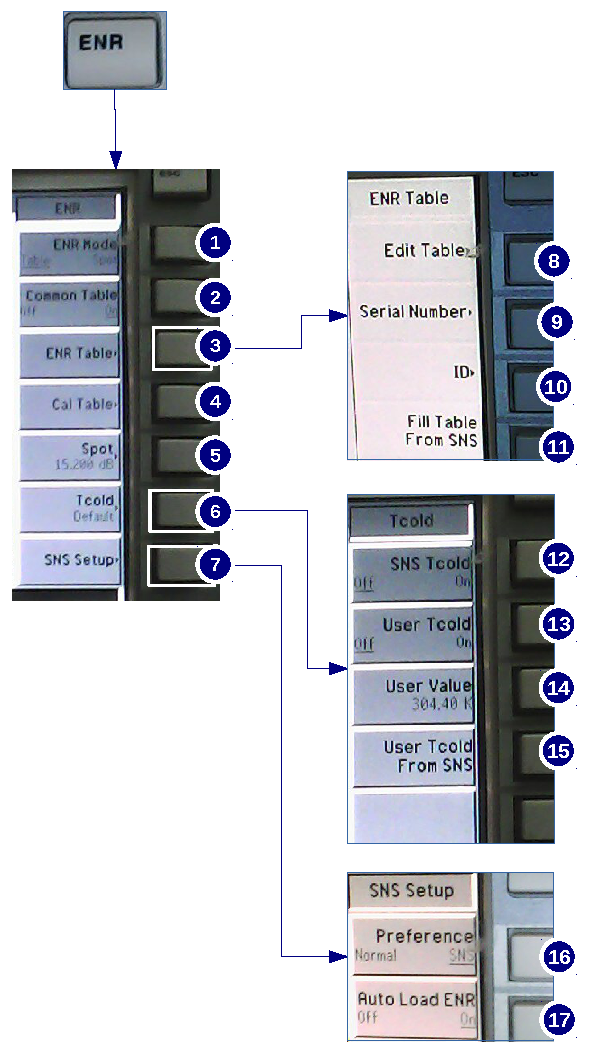
\includegraphics[width=0.5\textwidth]{./Imagenes/MenuENRN8975A.pdf}		
		\end{wrapfigure}
	
		\textbf{ENR}: permite introducir en el NFA \ todo lo relativo a los datos de la razón de excedente de ruido. Al presionar la tecla ENR del panel MEASURE se despliega en pantalla el menú de la figura 1. Se aprecia en la figura 1 que el NFA acepta los datos de ENR en formato tabular o en forma de valor
		puntual. El formato tabular le indica al equipo los valores de ENR para cada frecuencia de interés. En cambio se puede ingresar un único valor de ENR para ser utilizado en todo el rango de frecuencias de medición.	
		
		El equipo puede se configurado para aceptar dos tablas distintas de ENR al establecer la opción Common Table en Off. 
		
		El equipo puede aceptar dos tablas con datos de ENR, una de ellas se empleara exclusivamente en el durante el proceso de autocalibración (Cal Table) y la otra se usará para el proceso de medición ENR table.
		
		Cuando el modo de ENR esta establecido en Tabla, a través de las opciones y se pueden ingresar o editar las tablas de ENR para medición y calibración. Al presionar la tecla  espectiva, en pantalla se despliega el editor de tablas de ENR (figura). 	
		
		Cuando el modo ENR se configura en Spot, se ingresa un único valor de ENR con la opción de
		menú el cual se utilizara para todas las frecuencias de medición.
		
		A través del menú el usuario puede configurar el valor que empleará como temperatura física que posee la fuente de ruido, indicada en el menú como Tcold \ o temperatura fría. Al presionar esta opción, el usuario puede indicar si desea que el NFA cargue el valor de Tcold desde el sensor de temperatura de la fuente de ruido inteligente (SNS Tcold = On) o si debe tomar el valor establecido por el usuario (User Tcold = On). Cuando esta última opción esta activa, el usuario al presionar User Value y utilizando el teclado numérico puede ingresar el valor de Tcold o puede cargar el valor de Tcold desde la SNS
		
		El menu ENR permite establecer si el NFA empleará una fuente de ruido inteligente de la serie Agilent N4000 (SNS, serie N4000) o una fuente de ruido normal, serie 346 de Agilent. El NFA tiene la capacidad de cargar los datos de ENR de forma automatica cuando detecta	la conexión de una fuente de ruido SNS, con pción \ Auto Load ENR establecida en On.
	\end{minipage}
	
	\newpage		
	
	\begin{minipage}[t]{\textwidth}	
		\begin{wrapfigure}{r}{0.5\textwidth}	
			\centering	
			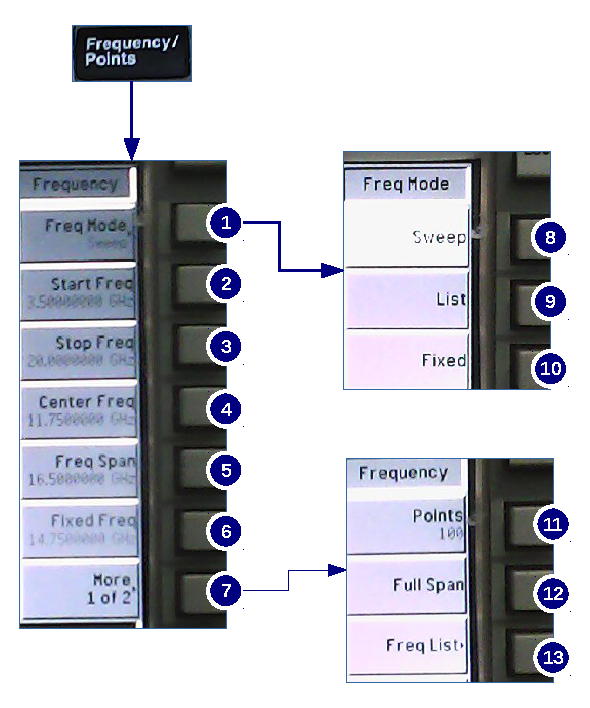
\includegraphics[width=0.5\textwidth]{Imagenes/MenuFrequencyPointsN8975A.pdf}	
		\end{wrapfigure}	
		
		\textbf{Frequency / Points} el NFA puede realizar mediciones sobre un rango de frecuencias, una lista de frecuencias oen una frecuencia puntual. Por medio de la opción Freq Mode se puede establecer que el NFA realize la medicion en forma	de barrido sobre un rango de frecuencias , sobre una lista de frecuencias, o en una frecuencia puntual (Fixed) 
		
		Cuando se utiliza el modo de barrido, el rango de frecuencias se especifica ya sea por su frecuencia de inicio y por su frecuencia final o bien por la frecuencia central del rango y su extensión. El numero de puntos \ que posee el rango se introduce con [Warning: Draw object ignored][Warning: Draw object ignored][Warning: Draw object ignored][Warning: Draw object ignored][Warning: Draw object ignored]Cuando se utiliza el modo de barrido, el rango de frecuencias se especifica ya sea por su frecuencia de inicio y por su frecuencia final o bien por la frecuencia central del rango y su extensión. El numero de puntos \ que posee el rango se introduce con 
				
		Cuando se establece el NFA que realice las mediciones sobre una lista de frecuencias, al presionar la
		opción, se muestra en pantalla el editor de lista de frecuencia sobre el cual el usuario ingresa los valores de frecuencia por medio del teclado numérico.][Warning: Draw object ignored][Warning: Draw object ignored]Cuando se establece el NFA que realice las mediciones sobre una lista de frecuencias, al presionar la opción, se muestra en pantalla el editor de lista de frecuencia sobre el cual el usuario ingresa los valores de frecuencia por medio del	teclado numérico.
		Cuando se desea medir en una frecuencia puntual, esta se ingresa por medio de la opción ][Warning: Drawobject ignored]Cuando se desea medir en una frecuencia puntual, esta se ingresa por medio de la opción. 		
	\end{minipage}
	
	\begin{minipage}[t]{\textwidth}
		\begin{wrapfigure}{l}{0.5\textwidth}	
			\centering	
			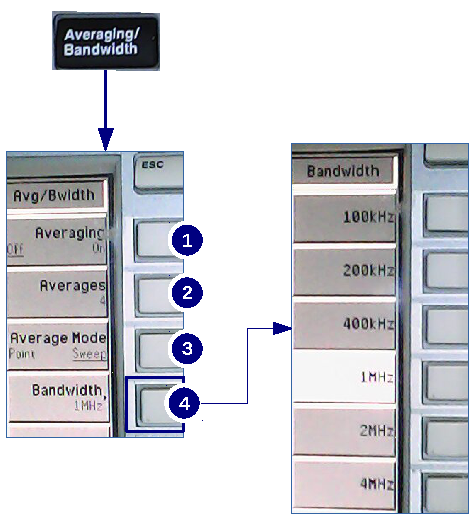
\includegraphics[width=0.5\textwidth]{Imagenes/MenuAverageBandwidthN8975A.pdf}	
		\end{wrapfigure}

		\textbf{Averaging / Bandwidth.} El promedio y el ancho de banda permite corregir los efectos del jitter del display en las mediciones. permite configurar el promedio y el ancho de banda. Para cada frecuencia de medición, el NFA mide la potencia de ruido en un ancho de banda centrado en torno a esta. El usuario puede elegir un valor para este ancho de banda de entre 6 opciones disponibles. El dispositivo puede ademas tomar múltiples mediciones y luego tomar el promedio de estas como el valor
		definitivo de la medición. Cuando se activa el promedio, el usuario puede especificar cuantas veces debe tomarse el mismo.	
		
		Al reducir el ancho de banda de medición, se incrementan los efectos del jitter en el display, lo cual puede corregirse incrementando el numero de promedios.
		
		Si se emplea un ancho de banda menor de 100 kHz, la cantidad de promedios debería ser 40 veces mayor si se desea obtener	la exactitud que se obtendría con un ancho de banda de 4 MHz.
		
		Si el promedio esta activo, el usuario puede seleccionar el modo de promedio (Average Mode) entre puntual (Point) \ o barrido (Sweep). Cuando se realiza el promedio puntual, el NFA calcula el promedio de	cada punto de frecuencia antes de avanzar al siguiente. Cuando el NFA ejecuta el promedio en barrido, el NFA realiza la	medición en un punto y avanza al siguiente. Cuando llega al ultimo punto, vuelve al primer punto toma una nueva medición y la promedia con el valor del último barrido, acumulando promedios en el tiempo. Esta opción permite ver el valor de la medicón en pantalla en tiempo real.
	\end{minipage}
	
	\begin{minipage}[t][11cm]{\textwidth}
		\begin{wrapfigure}{r}{0.5\textwidth}		
			\centering
			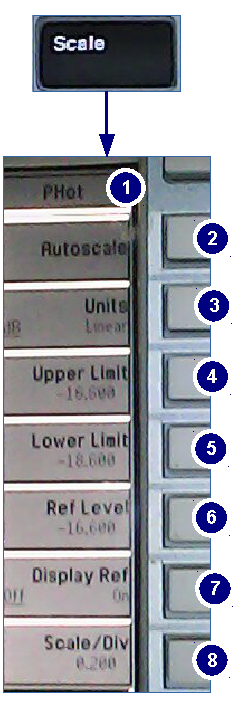
\includegraphics[height=10cm]{./Imagenes/MenuScaleN8975A.pdf}	
		\end{wrapfigure}
		
		\textbf{Scale.} Permite realizar ajustes relacionados a las escalas de los ejes en la presentación gráfica. La configuración de escala opera sobre el gráfico actualmente activo, se indica en el cual en la figura es un gráfico de PHot. Al presionar Autoscale la escala vertical de la gráfica activa se ajusta de modo automático para cubrir todo su rango de valores. Se puede seleccionar la unidad de presentación entre dB y lineal (Linear). \ Para la gráfica actualmente activa se puede ajustar los \ valores límites máximo y mínimo del eje vertical, así como también las unidades por división (Scale /
		Div).	
	\end{minipage}

	\begin{minipage}[t]{\textwidth}
		\begin{wrapfigure}{l}{0.5\textwidth}	
			\centering	
			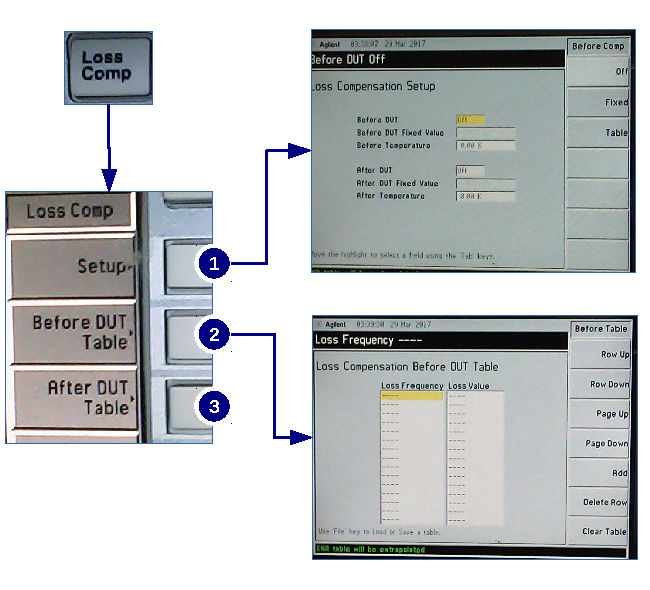
\includegraphics[width=0.5\textwidth]{Imagenes/MenuLossCompN8975A.pdf}	
		\end{wrapfigure}
		
		\textbf{Loss Comp.} permite realizar ajustes para compensar la atenuación y el ruido que	introducen los elementos presentes en el camino de señal, como cables y acopladores, ubicados antes y después del DUT. En la pantalla de edición se pude introducir un valor fijo de atenuación en los campos respectivos. También puede configurarse el equipo para aceptar o una tablas de valores de atenuación en función de la frecuencia en y luego ingresar las tablas de perdidas antes del DUT y después del DUT para las perdidas de los elementos antes y después del DUT. La pantalla cabia en este caso al modo de edición de tablas, donde se introduce un valor de frecuencia seguido de	su respectivo valor de perdidas.
		
		En se puede establecer la temperatura de ruido equivalente para los elementos antes o después del DUT. 
	\end{minipage}
	
	\begin{minipage}[t][10cm]{\textwidth}
		\begin{wrapfigure}{r}{0.5\textwidth}		
			\centering
			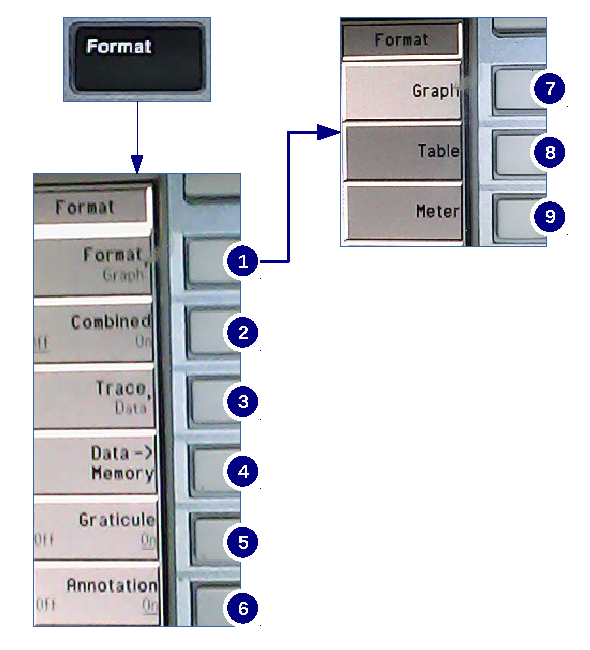
\includegraphics[width=0.5\textwidth, height=10cm, keepaspectratio]{./Imagenes/MenuFormatN8975A.pdf}	
		\end{wrapfigure}
		
		\textbf{Format.} Permite	seleccionar el formato de presentación de los datos de medición entre gráfico, tabla y valor puntual. Se \ puede activar la presentación de doble trazo en una única gráfica (Combined = On) o cada traza en su respectiva gráfica (Combined \ = Off), así como también activar la rejilla sobre los gráficos. 
		
		Pueden graficarse trazos almacenados en memoria del equipo, con y	
	\end{minipage}

	\begin{minipage}[t][10cm]{\textwidth}
		\begin{wrapfigure}{l}{0.5\textwidth}		
			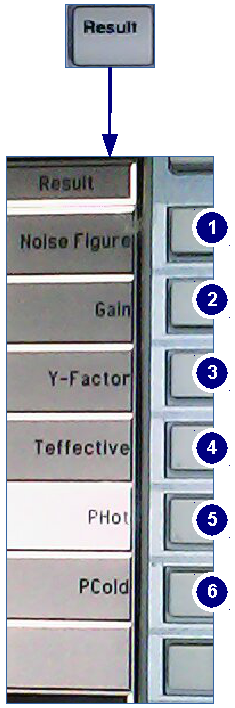
\includegraphics[width=0.5\textwidth, height=10cm, keepaspectratio]{./Imagenes/MenuResultN8975A.pdf}	
		\end{wrapfigure}
		
		\textbf{Result}: permite	elegir el valor de la medición que se visualiza en el gráfico activo, como la figura de ruido, la ganancia, el factor Y, la temperatura efectiva de ruido, la potencia de ruido “caliente” (fuente de ruido encendida) o la potencia de ruido fría.
	\end{minipage}



	%https://tex.stackexchange.com/questions/118602/how-to-text-wrap-an-image-in-latex
	%https://tex.stackexchange.com/questions/89821/how-to-draw-a-solid-colored-circle
	%https://tex.stackexchange.com/questions/96340/how-to-place-a-textnode-at-the-center-of-a-drawn-rectangle
	
	\begin{minipage}[t][11cm]{\textwidth}
		\begin{wrapfigure}{r}{0.5\textwidth}		
			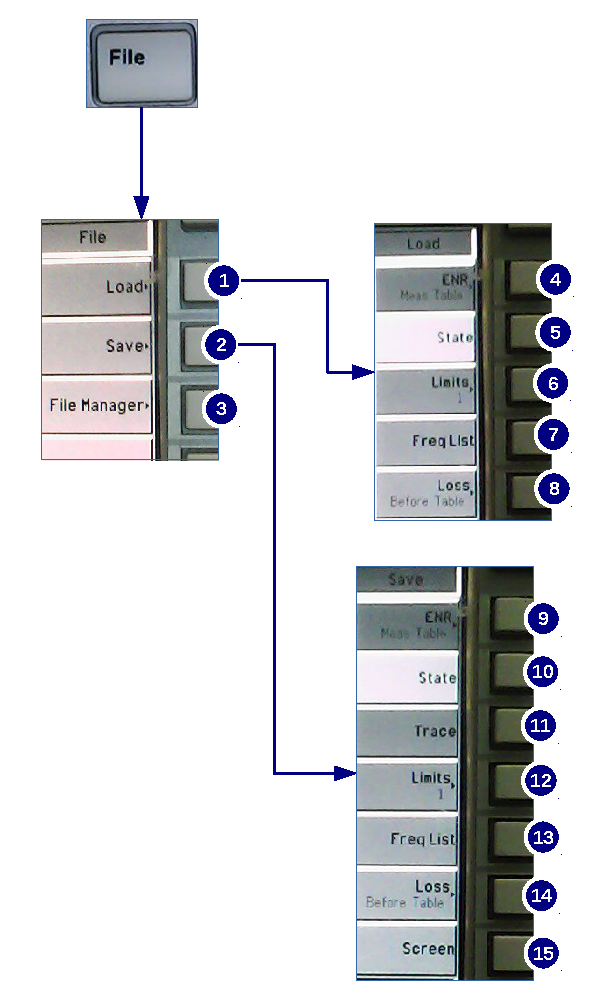
\includegraphics[width=0.5\textwidth, height=11cm, keepaspectratio]{./Imagenes/MenuFileN8975A.pdf}	
		\end{wrapfigure}		
		\textbf{File.} El N8975 posee la capacidad de almacenar información en su memoria interna o en un disco floppy, en forma de archivos. Al presionar la tecla File se presenta un menú con las funciones básicas sobre el sistema de archivos, Las opciones de menú permiten \ cargar (Load) y guardar (Save) archivos. La opción de menú , File Manager, presenta el administrador de archivos, por medio del cual se pueden copiar, renombrar y eliminar archivos, asi como también formatear un diskette en la unidad floppy.
		
		El N8975 puede almacenar o cargar archivos con tablas de ENR, estado del sistema, trazos limites, tablas de perdidas y gráficos desde o hacia la pantalla. 
	\end{minipage}


	\begin{minipage}[t][10cm]{\textwidth}
		\begin{wrapfigure}{l}{0.5\textwidth}		
			\centering
			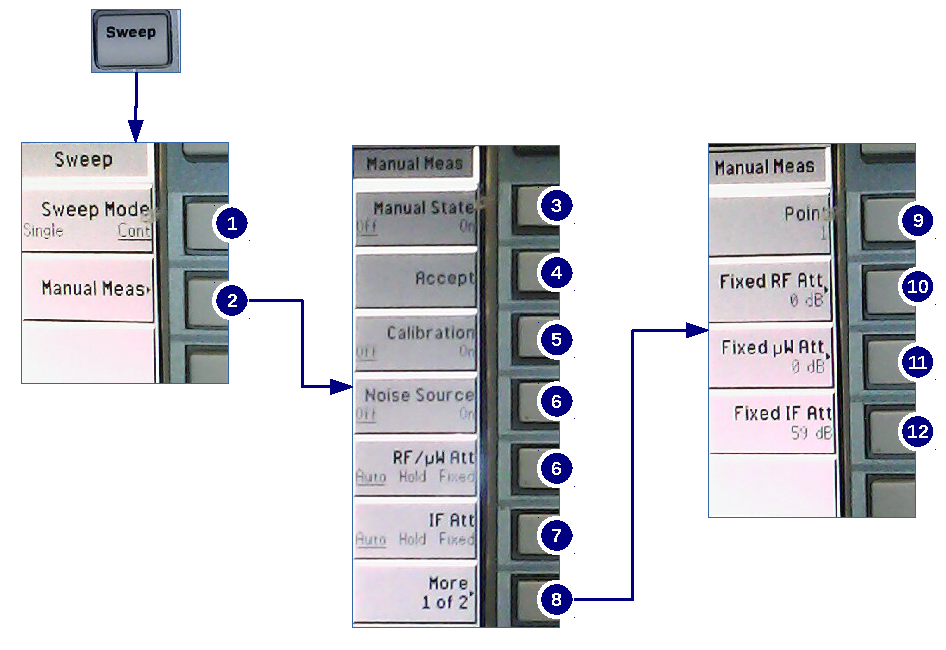
\includegraphics[width=0.5\textwidth]{./Imagenes/MenuSweepN8975A.pdf}	
		\end{wrapfigure}
		
		\textbf{Sweep.}		
	\end{minipage}
		
	Teclas de acción
	
	Al presionar se ejecuta un acción Calibrate, Full screen, Restart, Save Trace and Print.
	
	Capacidades del N8975
	
	Medición de potencia de ruido (PHOT, PCOLD~).
	
	Medición de Temperatura efectiva.
	
	Determinación del factor Y.
	
	Determinación de la figura de ruido.
	
	Medición de Ganancia.
	
	Puede ejecutar medidas en dispositivos simples o en sistemas de conversión de frecuencias.
	
	Mediciones básicas
	
	Preparación para proceso básico de medición
	
	Antes de realizar alguna medición de parámetros de ruido con el N8975, por lo general se deben ejecutar unos pasos
	previos de configuración del equipo.
	
	Para la medición de figura de ruido, el usuario debe ingresar ciertos datos al NFA antes de dar marcha con la medición.
	
	\begin{itemize}
		\item Ingresar los datos de la razón de ruido en exceso (ENR).
		\item Establecer el rango de frecuencias o la frecuencia individual sobre las cueles se desea la medida.
		\item Establecer el ancho de banda y configurar el promedio.
		\item Calibrar el analizador.
		\item Mostrar los resultados en pantalla.
	\end{itemize}

	Ingresar datos de ENR
	
	[Warning: Draw object ignored]El NFA requiere los datos de ENR de las fuentes de ruido que se utilicen durante las
	mediciones. El equipo emplea los valores de ENR en dos situaciones distintas: \ durante el proceso de auto-calibración
	y durante la medición de figura de ruido. Cuando el equipo ejecuta la auto-calibración, éste emplea una tabla de
	valores ENR de la fuente de ruido con la cual se lleva acaba este ajuste, por medio del cual el equipo elimina su
	contribución de ruido en la medición. Durante la medición de figura de ruido, el equipo emplea los datos de ENR de la
	fuente de ruido y mediciones directas de potencia de ruido para calcular y presentar en pantalla el valor F. 
	
	El N8975 admite el ingreso de los datos ENR se ingresan al N8975 en forma de tabla o en forma de valor puntual (spot
	value). \ Para el formato tabla, cada fila de esta consiste en un par de valores, frecuencia y ENR, esta tabla se
	emplea para medición en múltiples frecuencias. Si el equipo necesita el valor de ENR en alguna frecuencia que no este
	listado en esta tabla, simplemente calculará el valor que necesita por interpolación. \ Esto ocurre cuando la
	configuración establecida por el usuario para la frecuencia máxima, frecuencia \ mínima \ y cantidad de puntos de
	medición provocan que el rango de frecuencias sobre el cual medirá el NFA no concuerde con las frecuencias de la tabla
	ENR. 
	
	Debería medirse el DUT a las mismas frecuencias que establece la tabla de ENR de la fuente de ruido.
	
	Cuando se ingresa un valor puntual de ENR, el equipo lo emplea para medición en una sola frecuencia \ es aplicado en
	todo todo el rango de medición.
	
	El equipo puede operar con \ dos tablas distintas para ENR: una tabla para ENR de calibración \ y una tabla para valores
	de ENR de medición. La tabla ENR de calibración la emplea el equipo cuando ejecuta el proceso de auto-calibración. La
	tabla ENR de medición la emplea el equipo \ durante la medición de figura de ruido. \ 
	
	Puede configurarse el equipo para que utilice dos tablas de ENR distintas (calibración y medición) o para que utiliza
	una única tabla de ENR, la tabla ENR de calibración, para la tarea de auto calibración y medición de figura de ruido.
	
	La utilidad en emplear dos tablas de ENR esta en que se puede emplear una fuente de ruido para el proceso de
	auto-calibración y otra fuente de ruido distinta para el proceso de medición. 
	
	La fuentes de ruido normales, como las \ Agilent 346, el usuario debe ingresar \ de forma manual o por medio de un
	diskette que le suministra el fabricante los datos de ENR, el fabricante suministra estos datos. La fuentes de ruido
	inteligentes de Agilent (SNS) pueden cargar los datos de ENR de manera automática al NFA.
	
	Los puntos de frecuencia a medir son determinados por entradas en la tabla de ENR?
	
	Los datos de ENR pueden cargarse de cuatro formas distintas maneras:
	
	\begin{itemize}
		\item Se puede ingresar un único valor de THOT
		\item Puede introducir datos de ENR por medio de un disco floppy, en donde previamente se haya almacenado la data de
		Introduciéndolo en la ranura que dispone el NFA y utilizando el administrador de archivos. Se accede a las funciones e
		control de archivos por medio del botón File (panel System).
		\item Puede cargar los datos desde la memoria interna del NFA. 
		\item Puede cargar los datos de forma remota, a través del bus GPIB. 
		\item En caso de utilizar una fuente de ruido inteligente, como las Agilent serie N4000, el usuario puede elegir si
		cargar de foma automática cuando se conecte una fuente de ruido.
	\end{itemize}
	Ingresar datos de temperatura (TCOLD)
	
	En caso de que la temperatura en el recinto donde se efectúe la medición sea distinta a la temperatura por defecto
	establecida en el equipo de 296.05K, se debe ingresar al equipo el valor de la temperatura (TCOLD). Cuando se emplean
	las fuentes de ruido inteligentes SNS, serie Agilent N4000, este paso puede \ ya que estas fuentes incluyen un sensor
	de temperatura interno, el NFA puede cargar automaticamente el valor de temperatura correcto al momento de efectuar
	cada medición.
	
	Establecer las frecuencias de medición
	
	El usuario debe establecer el conjunto de frecuencias sobre las cuales se realizará la medida. El N8975 dispone de tres
	opciones para la selección de frecuencias de medición: barrido (swep), lista (list) y fija (fixed).
	
	Barrido (sweep): el rango de frecuencias de medición se obtiene de una frecuencia inicial, una frecuencia final y el
	numero de medidas.
	
	Lista (list): las frecuencias de medición se especifican ingresando en el N8975 una lista de valores de frecuencia.
	
	Fija (fixed): el usuario establece que la medición se realizará en un único valor de frecuencia.
	
	Establecer el ancho de banda y activación del promedio.
	
	Se selecciona un valor para el \ ancho de banda, el cual determina \ en torno a cada valor de frecuencia sobre el cual
	se integra la potencia de ruido. El usuario debe escogen un valor de ancho de una lista, las opciones para el ancho de
	banda son \ 100 kHz, 200 kHz, 400 kHz, 1 MHz, 2Hz y 4MHz.
	
	El usuario puede elegir si desea activar el promedio en las mediciones. Si se activa el proedio, puede establecer si es
	un promedio puntual o promedio de barrido.
	
	Al activar el promedio el jitter y se provee de mediciones más precisas cuanto más promedios se realice. Sin embargo, la
	velocidad de medición se reduce.
	
	Calibración
	
	Cumplidos los pasos anteriores, se ejecuta la auto calibración del equipo N8975. La auto calibración le permite a este
	equipo compensar la contribución de ruido introducida por el cableado y accesorios que se encuentren en el camino de
	señal además del ruido generado por el propio N8975.		
	
	\begin{figure}
		\centering
		\begin{minipage}{8.063cm}
			%\includegraphics{Imagenes/EsquemaConexionCalibracion.png}
			\caption{Conexión del sistema para ejecutar auto calibración.}
		\end{minipage}
	\end{figure}
	Se conecta el equipo con indica la figura. Los datos de ENR para la fuente de ruido empleada en la calibración deben haberse introducido previamente en la tabla de calibración.
			
	Mostrar resultados
	
	El equipo puede presenta los resultados en forma de gráficos, tabla o valor textual. En cuanto a la presentación de	gráficos, el equipo puede presentar dos resultados en pantalla de manera simultanea o combinarlos en un mismo gráfico. Puede salvar la gráfica activa en memoria.
	
	Interruptor mecánico de 3GHz
	
	El NFA N8975 posee un interruptor mecánico ajustado para conmutar del rango de frecuencia de 10 MHz a 3.0 GHz al rango	de 3.0GHz a 26.5GHz. Si el rango de frecuencia que seleccione el usuario cruza el punto de 3.0GHz, el switch mecánico se activa. El interruptor mecánico tiene un un numero limitado de activaciones sobre el cual es confiable. La	conmutación sobre los 3.0 GHz debe limitarse siempre que sea posible
	
	Antes de emplear el N2002A debe realizarse un test de verificación, para asegurar que los caminos de conmutación	funcionen y que el VSWR este dentro de los limites [1.19]	
